\documentclass[MASTER.tex]{subfiles}
\begin{document}
%================================================================================================%
\begin{frame}[fragile]
\frametitle{Poisson Regression with \texttt{R}}
\Large 
\textbf{glm} function output
\begin{itemize}
 \item The output begins with echoing the function call. Then the information on deviance residuals is displayed. 
 \item Deviance residuals are approximately normally distributed if the model is specified correctly.
 \item Here it shows a little bit of skeweness since median is not quite zero. 
\end{itemize}
\end{frame}
%================================================%
\begin{frame}
\Large 
\textbf{glm} function output
\begin{itemize}
\item The Poisson regression coefficients for each of the variables along with the standard errors, z-scores, p-values 
and 95\% confidence intervals for the coefficients. 
\item The coefficient for math is 0.07.
\item This means that the expected log count for a one-unit increase in math is 0.07. 
\end{itemize}
\end{frame}
%============================================================================ %
\begin{frame}[fragile]
\frametitle{Poisson Regression with \texttt{R}}
\begin{verbatim}
Coefficients:
			Estimate Std. Error z value Pr(>|z|)    
(Intercept)     -5.2471     0.6585   -7.97  1.6e-15 ***
progAcademic     1.0839     0.3583    3.03   0.0025 ** 
progVocational   0.3698     0.4411    0.84   0.4018    
math             0.0702     0.0106    6.62  3.6e-11 ***
	---
Signif. codes:  0 '***' 0.001 '**' 0.01 '*' 0.05 '.' 0.1 ' ' 1
			
\end{verbatim}
\end{frame}

%===========================================================%
\begin{frame}[fragile]
\frametitle{Poisson Regression with \texttt{R}}
\Large 
\textbf{glm} function output
	\begin{itemize}

\item The indicator variable \textbf{progAcademic} compares between \textbf{\textit{prog = “Academic” }}and \textbf{\textit{prog = ``General"}} , the expected log 
count for \textbf{\textit{prog = “Academic” }}increases by about 1.1. \smallskip
\item The indicator variable \textbf{prog.Vocational}  is the expected difference in log count (\(\approx 0.37\)) between 
\textbf{\textit{prog = "Vocational"}} and the reference group (\textbf{\textit{prog = "General"}} ).
\end{itemize}
\end{frame}
%================================================================================================%
\begin{frame}[fragile]
\frametitle{Poisson Regression with \texttt{R}}
	\Large 
	\begin{itemize}
		\item The output above indicates that the incident rate for \textbf{prog = ``Academic"} is 2.96 times the incident rate for the reference group (\textbf{prog = "General"}). 
		\item Likewise, the incident rate for \textbf{prog = ``Vocational"} is 1.45 times the incident rate for the reference group holding the other variables at constant. 
		
	\end{itemize}
	
\end{frame}
%================================================================================================%
\begin{frame}[fragile]
\frametitle{Poisson Regression with \texttt{R}}
	\Large 
	\begin{itemize}
		\item
		The percent change in the incident rate of \textbf{num\_awards} is by 7\% for every unit increase in math. 
		% For additional information on the various metrics in which the results can be presented, and the interpretation of such, please see Regression Models for Categorical Dependent Variables Using Stata, Second Edition by J. Scott Long and Jeremy Freese (2006).
	\end{itemize}
\end{frame}
%===========================================================%
\begin{frame}[fragile]
\frametitle{Poisson Regression with \texttt{R}}
\Large 
\textbf{Deviance}
\begin{itemize}
\item In statistics, deviance is a quality of fit statistic for a model that is often used for statistical hypothesis testing. 
\item It is a generalization of the idea of using the sum of squares of residuals in ordinary least squares to cases where model-fitting is achieved by maximum likelihood.
\end{itemize}
\end{frame}
%===========================================================%
\begin{frame}[fragile]
\frametitle{Poisson Regression with \texttt{R}}
\Large 
\textbf{glm} function output
\begin{itemize}
\item The information on deviance is also provided. 
\item We can use the residual deviance to perform a goodness of fit test for the overall model. 

\end{itemize}
\end{frame}
%===========================================================%
\begin{frame}[fragile]
\frametitle{Poisson Regression with \texttt{R}}
\Large 
\textbf{glm} function output
\begin{itemize}
\item The residual deviance is the difference between the deviance of the current model and the maximum deviance of the ideal model where the predicted values are identical to the observed. \smallskip
\item Therefore, if the residual difference is small enough, the goodness of fit test will not be significant, indicating that the model fits the data. 
%\item We conclude that the model fits reasonably well because the goodness-of-fit chi-squared test is not statistically significant.

%\item \textbf{REMARK:} Model Appraisal for GLMs subject of future talk.
\end{itemize}
\end{frame}
%===========================================================%
\begin{frame}[fragile]
\frametitle{Poisson Regression with \texttt{R}}
\Large 
\textbf{glm} function output
\begin{itemize}
\item If the test had been statistically significant, it would indicate that the data do not fit the model well. 
\item We could try to determine if there are omitted predictor variables, if our linearity assumption holds and/or if there is an issue of over-dispersion. 
\end{itemize}
\end{frame}

%================================================================================================%
%\begin{frame}[fragile]
%
%\frametitle{Poisson Regression with \texttt{R}}
%\large
%
%\begin{framed}
%\begin{verbatim}
%with(m1, cbind(res.deviance = deviance, 
%	df = df.residual,
%        p = pchisq(deviance, df.residual, 
%            lower.tail=FALSE)))
% 
%      res.deviance  df      p
% [1,]        189.4 196 0.6182
%\end{verbatim}
%\end{framed}
%\end{frame}

%================================================================================================%
\begin{frame}[fragile]

\frametitle{Poisson Regression with \texttt{R}}
\Large 
\textbf{Comparing Candidate Models}
\begin{itemize}
\item 
We can also test the overall effect of prog by comparing the deviance of the full model with the deviance of the model 
excluding prog.
\item The two degree-of-freedom chi-square test indicates that prog, taken together, is a statistically significant predictor of \textbf{num\_awards}.
\end{itemize} 

\end{frame}

%================================================================================================%
\begin{frame}[fragile]

\frametitle{Poisson Regression with \texttt{R}}
\large
\textbf{Comparing Models}
\begin{framed}
\begin{verbatim}
# update m1 model dropping prog
m2 <- update(m1, . ~ . - prog)

# test model differences with chi square test
anova(m2, m1, test="Chisq")
\end{verbatim}
\end{framed}
\end{frame}


%================================================================================================%
\begin{frame}[fragile]
\frametitle{Poisson Regression with \texttt{R}}
\begin{verbatim}
 Analysis of Deviance Table
 
 Model 1: num_awards ~ math
 Model 2: num_awards ~ prog + math
   Resid. Df Resid. Dev Df Deviance Pr(>Chi)    
 1       198        204                         
 2       196        189  2     14.6  0.00069 ***
 ---
 Signif. codes:  0 '***' 0.001 '**' 0.01 '*' 0.05 '.' 0.1 ' ' 1
\end{verbatim}

\end{frame}

%================================================================================================%
\begin{frame}[fragile]
\frametitle{Poisson Regression with \texttt{R}}
\Large 
\textbf{Incident Rate Ratios}
\begin{itemize}
\item Sometimes, we might want to present the regression results as \textbf{incident rate ratios} (IRRs) and 
their standard errors, together with the confidence interval. 
\item To compute the standard error for the incident rate ratios, we will use the \textbf{Delta method} ( Numerical Computation Method). 
\item To this end, we make use the function \texttt{deltamethod} implemented in R package \textbf{msm}.
\end{itemize}
\end{frame}
%================================================================================================%
\begin{frame}[fragile]
	
	\frametitle{Poisson Regression with \texttt{R}}
	\Large 
	\textbf{Incident Rates} \\
	Incidence rate is the occurrence of an event over person-time, for example person-years.
	
	\[ \mbox{Incidence Rate}  = \frac{\mbox{events}}{\mbox{Person Time}} \]
	\smallskip
	Note: the same time intervals must be used for both incidence rates.
\end{frame}
%===================================================%
\begin{frame}[fragile]
\frametitle{Poisson Regression with \texttt{R}}
\Large 
\textbf{Incident Rate Ratios}\\
A \textbf{rate ratio} (sometimes called an incidence density ratio) in epidemiology, is a relative difference measure used to compare the incidence rates of events occurring at any given point in time. %A common application for this measure in analytic epidemiologic studies is in the search for a causal association between a certain risk factor and an outcome.
\smallskip
\[ \mbox{Incidence Rate Ratio }  = \frac{\mbox{Incidence Rate 1}}{\mbox{Incidence Rate 2}} \]
\end{frame}
%================================================================================================%

%================================================================================================%
\begin{frame}[fragile]

\frametitle{Poisson Regression with \texttt{R}}
\textbf{Delta Method}

\begin{verbatim}
s <- deltamethod(list(~ exp(x1), ~ exp(x2), ~ exp(x3), 
      ~ exp(x4)), coef(m1), cov.m1)

#exponentiate old estimates dropping the p values

rexp.est <- exp(r.est[, -3])

# replace SEs with estimates 
# for exponentiated coefficients

rexp.est[, "Robust SE"] <- s

\end{verbatim}

\end{frame}

%================================================================================================%
\begin{frame}[fragile]

\frametitle{Poisson Regression with \texttt{R}}

\begin{framed}
\begin{verbatim}
rexp.est
 
                Estimate Robust SE       LL      UL
 (Intercept)    0.005263   0.00340 0.001484 0.01867
 progAcademic   2.956065   0.94904 1.575551 5.54620
 progVocational 1.447458   0.57959 0.660335 3.17284
 math           1.072672   0.01119 1.050955 1.09484
\end{verbatim}
\end{framed}
\end{frame}


%================================================================================================%
\begin{frame}[fragile]

\frametitle{Poisson Regression with \texttt{R}}
\Large
\begin{itemize}
\item Sometimes, we might want to look at the expected marginal means. 
\item For example, what are the expected counts for each program type holding math score at its overall mean? 
\item To answer this question, we can make use of the predict function. 
\item First off, we will make a small data set to apply the predict function to it.
\end{itemize}

\end{frame}

%================================================================================================%
\begin{frame}[fragile]

\frametitle{Poisson Regression with \texttt{R}}
\normalsize 

\begin{framed}
\begin{verbatim}
(s1 <- data.frame(math = mean(p$math),
  prog = factor(1:3, levels = 1:3, 
  labels = levels(p$prog))))
 
    math       prog
 1 52.65    General
 2 52.65   Academic
 3 52.65 Vocational
\end{verbatim}
\end{framed}
\end{frame}

%================================================================================================%
\begin{frame}[fragile]

\frametitle{Poisson Regression with \texttt{R}}
\normalsize 

\begin{framed}
\begin{verbatim}
predict(m1, s1, type="response", se.fit=TRUE)
 
 $fit
      1      2      3 
 0.2114 0.6249 0.3060 
 
 $se.fit
       1       2       3 
 0.07050 0.08628 0.08834 
 
 $residual.scale
 [1] 1
\end{verbatim}
\end{framed}
\end{frame}

%================================================================================================%
\begin{frame}[fragile]

\frametitle{Poisson Regression with \texttt{R}}
\Large 
\begin{itemize}
\item 
In the output above, we see that the predicted number of events for level 1 of prog is about 0.21, holding math at its mean.
\item The predicted number of events for level 2 of prog is higher at 0.62, and the predicted number of events for level 
3 of prog is about .31. 
\item The ratios of these predicted counts (\(\frac{0.625}{0.211} = 2.96\), \(\frac{0.306}{0.211} = 1.45\)) match what 
we saw looking at the IRR.
\end{itemize}
\end{frame}


\begin{frame}

\begin{figure}
\centering
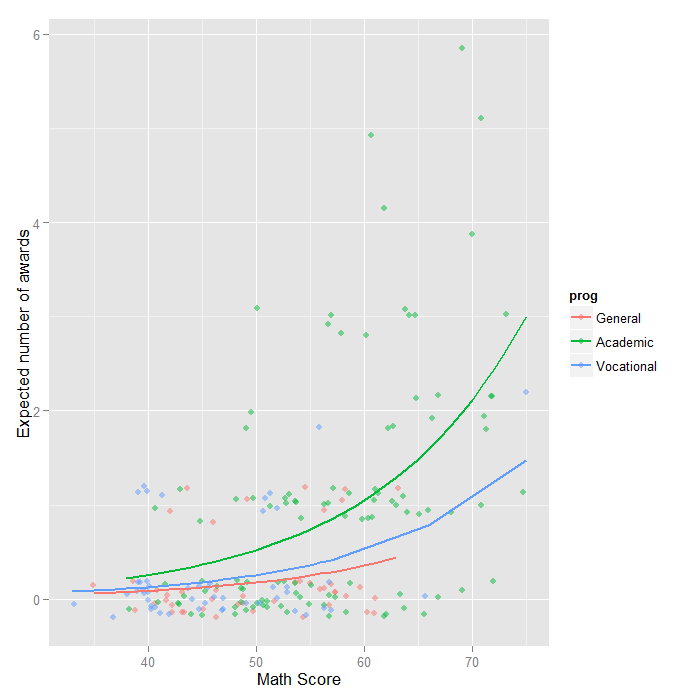
\includegraphics[width=0.85\linewidth]{poisson2}
%\caption{}
%\label{fig:poisson2}
\end{figure}

\end{frame}
%================================================================================================%
%\begin{frame}[fragile]
%--------- PLOTTING
% -------- CUT NEXT THREE SLIDES
%\frametitle{Poisson Regression with \texttt{R}}
%\Large
%
%\begin{itemize}
%\item We can also graph the predicted number of events with the commands below. 
%\item The graph indicates that the most awards are predicted for those in the academic program (prog = 2), 
%especially if the student has a high math score. 
%\item The lowest number of predicted awards is for those students in the general program (prog = 1). 
%\item The graph overlays the lines of expected values onto the actual points, although a small amount of random noise was added vertically to lessen overplotting.
%\end{itemize}
%\end{frame}
%
%%================================================================================================%
%\begin{frame}[fragile]
%
%\frametitle{Poisson Regression with \texttt{R}}
%\Large
%
%\begin{framed}
%\begin{verbatim}
%# Calculate and store predicted values
%p$phat <- predict(m1, type="response")
%
%# order by program and then by math
%p <- p[with(p, order(prog, math)), ]
%\end{verbatim}
%\end{framed}
%\end{frame}
%%================================================================================================%
%\begin{frame}[fragile]
%
%\frametitle{Poisson Regression with \texttt{R}}
%\large
%% create the plot
%
%\begin{framed}
%\begin{verbatim}
%ggplot(p, aes(x = math, y = phat, colour = prog)) +
%  geom_point(aes(y = num_awards), alpha=.5, position=position_jitter(h=.2)) +
%  geom_line(size = 1) +
%  labs(x = "Math Score", y = "Expected number of awards")
%\end{verbatim}
%\end{framed}
%\end{frame}
%======================================================


\end{document}
